\subsection{Limitations of Perceptrons}

\mode<article>{
Connectionist neurons, or perceptrons, are limited in the variety of functions they are able to fit. 
When dealing with classification problems, a perceptron can only find a linear separation between any two classes. Irrespective of the neuron's non-linear activation function, the perceptron is regarded as a \emph{linear classifier}. Whether something falls on one side of the decision boundary or the other, is entirely based on applying a linear filter $\vec w^{\top} \vec x$. The non-linearity $f(h)$ merely controls the value range of the neuron's response ($\{0,1\}, (-1,+1)$, \ldots) which helps in intepreting the neuron's response.\\

If observations from two different classes are dsitributed such that one cannot draw a line to separate them, then the two classes
are not linearly separable. In this case the perceptron will fail to find a suitable classification boundary between the two classes.
}

\begin{frame}\frametitle{Linear classifiers/linear decision boundaries}

Consider the following binary classification problems with $\vec x \in \R^2$.{}

\question{Can you find a line that separates the two classes for each case? Do you recognize the function described in each?}

\begin{figure}[h]
    \centering
	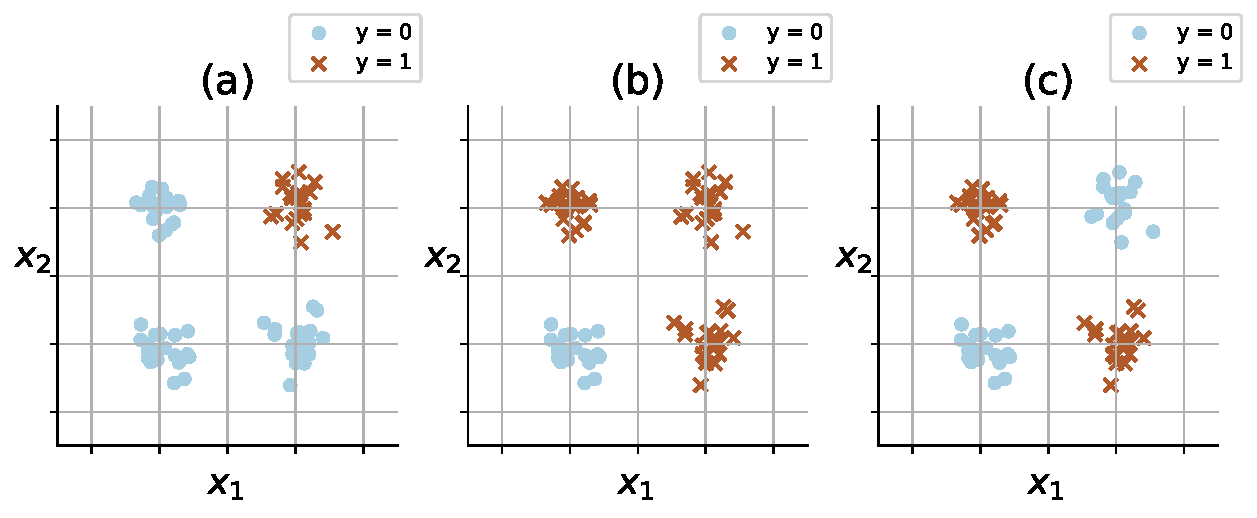
\includegraphics[width=0.8\textwidth]{img/and_or_xor_y}
	\mode<article>{
	\caption{(a) points are classified according to the AND function,
	(b) points are classified according to the OR function,
	(c) points are classified according to the XOR function.
	}
	}
	\label{fig:and_or_xor} 
\end{figure}

\mode<article>{
In \figureref{fig:and_or_xor}, particularly (a) and (b),
it is possible to draw a line that separates the classes. Therefore, the AND and OR functions are linearly separable.
A perceptron is capable of finding such a separating line. This does not apply to the case in (c), which is the XOR function.
It is impossible to find a single line that will separate the classes. The data from the XOR function is not linearly separable.
}

\pause

\question{Can we solve the XOR problem with multiple perceptrons? How?}

\notesonly{
- Yes, Think of it as a divide and conquer approach. We split the XOR problem into mulitple sub-problems. 
A perecptron is used to solve each sub-problem.

If you're familiar with boolean algebra, you might reocgnize the following expression for the XOR function:
}

\end{frame}

\begin{frame}\frametitle{Solving the XOR problem}

\begin{equation}
\label{eq:xor}
\mathrm{XOR}(x_1, x_2) = 
(
\underbrace{
{\color{magenta}\,{x_1} \; \mathrm{AND} \; \overline{x}_2 \,}
}_{=:{\color{magenta}s^1_1}}
)
 \;\; \mathrm{OR} \;\; 
(
\underbrace{
{\color{green}\, \overline{x}_1 \; \mathrm{AND} \; x_2 \,}
}_{=:{\color{green}s^1_2}}
)
\end{equation}

\mode<article>{
For instance, the first perceptron ${\color{magenta}s^1_1}$ is tasked to separate the bottom-right cloud of points from the rest. The meaning of the indices around the "S" will be clarified shortly.
A second perceptron ${\color{green}s^1_2}$ is used to separate the top-left cloud from the rest. 
A third perceptron $s^2_1$ will use the responses from of the first two perceptrons as its input. It will then respond to ``is \emph{only one} of the previous two perceptrons ON?''.

\figureref{fig:build_xor} illustrates this approach. One need only recognize that each sub-problem is linearly separable.\\
}

\end{frame}
\begin{frame}

\begin{figure}[ht]
    \centering
	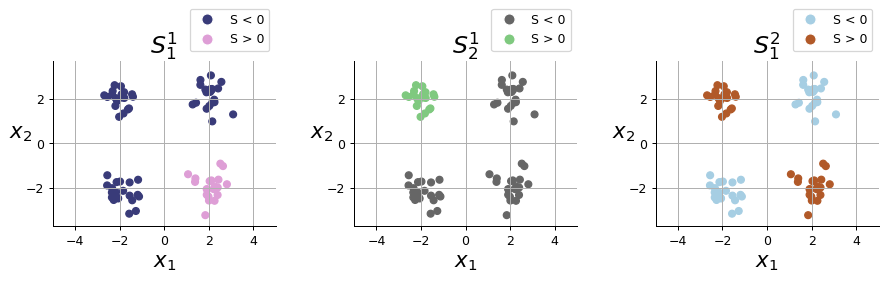
\includegraphics[width=0.55\textwidth]{img/build_xor.png}
	\caption{Solving sub-problems of the XOR problem.}
	\label{fig:build_xor} 
\end{figure}

\end{frame}

\mode<article>{
What we are essentially describing is a Multilayered perceptron (MLP) with an architecture as illustrated in \figref{fig:xor_mlp_arch}. The MLP is made up of an output layer with  a single output neuron $S^2_1$, and one hidden layer with two hidden neurons, $S^1_1$ and $S^2_2$ (the superscript denotes the layer index, the subscript denotes the neuron index within its layer). The terms ``neurons'' and ``nodes'' will be used interchangeably and synonymously.
}

\begin{frame}

\begin{figure}[h]
    \centering
	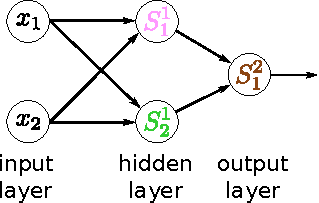
\includegraphics[width=0.5\textwidth]{img/xor_mlp_arch}
	\caption{MLP architecture for the XOR problem consisting of one hidden layer with two hidden nodes $s^1_1$, $s^1_2$, and one output layer with a single output neuron $S^2_1$}
	\label{fig:xor_mlp_arch} 
\end{figure}

\end{frame}
